\subsection{OpenShift infrastructure}\label{subsec:openshift-infrastructure}

These group of tasks manage the creation and configuration of an OpenShift infrastructure.
This infrastructure can then be used to test the releases for the marketplaces using CSVs and OLM.
In general these tasks do not have to run for every release, but can be used to debug one should errors arise.

\begin{figure}[H]
    \centering
    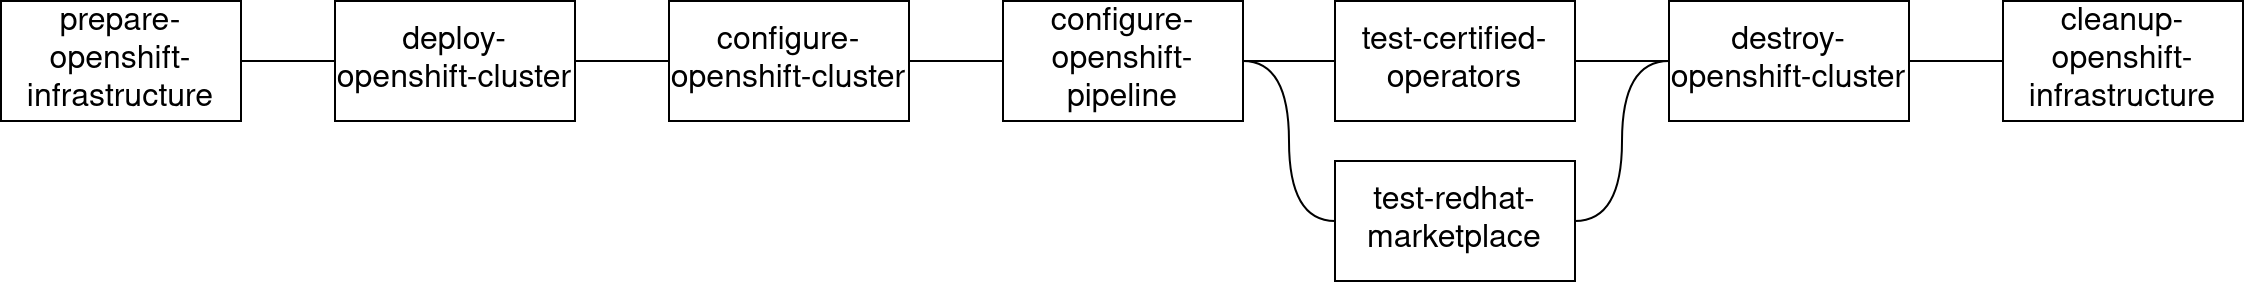
\includegraphics[width=\textwidth]{img/implementation/openshift}
    \caption{Pipeline to maintain OpenShift infrastructure.}
    \label{fig:pipeline-to-maintain-openshift-infrastructure}
\end{figure}

In Figure~\ref{fig:pipeline-to-maintain-openshift-infrastructure} the structure of these tasks is displayed.
Since they can run independently of the main release tasks, they are detached from them.
At the start of the pipeline, the OpenShift cluster is created.
Then the releases for the marketplaces using CSVs can be tested.
Since not all four releases using CSVs are different, only two types of tests exist.
Afterwards, the infrastructure can be destroyed again.

\subsection{Prepare OpenShift infrastructure}\label{subsec:prepare-openshift-infrastructure}

The purpose of this task it to prepare an S3 bucket for the Openshift installer to place a state file in.
This task creates an S3 bucket to place openshift installer state into.
It uses a python script to do so.
This script takes the parameters shown in table \ref{tab:parameters-to-create-an-s3-bucket}.

\begin{table}[H]
    \centering
    \caption{Parameters to create an S3 bucket}
    \label{tab:parameters-to-create-an-s3-bucket}
    \begin{tabular}{p{0.3\linewidth}|p{0.6\linewidth}}
        Parameter & Expected value \\
        \hline
        \verb| --cluster-name | & The name of the cluster which will be created.
            It is usually the same name as the pipeline. \\
        \verb| --bucket-name | & The name the created bucket should have. \\
        \verb| --bucket-region | & The AWS region the bucket should be created in. \\
        \verb| --remove | & A flag to remove an existing bucket again \\
    \end{tabular}
\end{table}

The \verb| boto3 | python library is then used to connect to AWS S3 service.
If the given bucket name does not exist, it is created and an empty file is uploaded as a state file.
If the given bucket name does exist, but a state file is missing, an empty file is created and uploaded.


\subsection{Deploy OpenShift cluster}\label{subsec:deploy-openshift-cluster}

This task deploys an Openshift cluster on AWS infrastructure.
First, it checks if a state file exists in the S3 bucket created in the previous task.
The file is then unzipped.
If a install configuration already exists in this file, the installation was already done and the current one is skipped.

Otherwise, Openshift is installed.
First, a new install configuration file is created, based one the \verb|{install_config}| parameter.
In it, the AWS region and the cluster name, which are configured with the \verb|{aws_region}| and \verb|{cluster_name}| respectively, are set.

Downloading the Openshift installer is done in one of two ways.
First, by setting a installer URL.
If this URL is set, the Openshift installer is downloaded from the URL and the script assumes it is a binary.
This way of downloading the Openshift installer is not tested, therefore there is no parameter provided to set the installer URL.

The second way of downloading Openshift, which is supported by the pipeline, is by defining the target version, URL to the Openshift installer directory and whether unstable versions should also be considered or not.
Configuring these values is done with the \verb|{ocp_version}|, \verb|{ocp_installer_directory_url}|, and \verb|{ocp_installer_unstable}| parameters respectively.
The task then downloads the latest patch version of the installer and extracts the downloaded archive containing the installer.
After the installer has been downloaded, it is executed to create the cluster.

When the installer has finished, the deployments VPCs are queried, along with their security groups and NAT gateways.
These VPCs and gateways are then whitelisted AWS's infrastructure.
The installer state, which was written by the installer, is then zipped and uploaded to the S3 bucket.
Finally, the resulting \verb|kubeconfig| is saved as a Vault secret under the name of \verb|openshift|.



# configure-openshift-cluster

This task, like `prepare-openshift-infrastructure` and `deploy-openshift-cluster`, was taken from the repository [pipeline-cpn-kubernetes](https://bitbucket.lab.dynatrace.org/projects/CPN/repos/pipeline-cpn-kubernetes/browse) repository.
It labels nodes and can update the openshift version, if the `{ocp_channel}` has changed.

## Purpose

Minor setup of nodes and updating Openshift.

## Configuration options

The parameters can be changed in the [params-dev](../../params-dev.yaml) or [params-prod](../../params-prod.yaml) files.
The following parameters can be used to configure this task.

| Parameter   | Effect                                                                         | Production default | Development default |  | Production default | Development default |
| ----------- | ------------------------------------------------------------------------------ | ------------------ | ------------------- |
| ocp_channel | Defines which release channel of Openshift should be used to check for update. | `stable`           | `stable`            |

## Common error cases

This task usually only fails if the S3 bucket does not exist. 
I.e., if the previous tasks were not run in the correct order or if `cleanup-openshift-infrastructure` ran in the mean time.
The correct order of tasks is as follows.

1. prepare-openshift-infrastructure
2. deploy-openshift-cluster
3. configure-openshift-cluster
4. configure-openshift-pipeline
5. Optional:
   * test-certified-operators
   * test-redhat-marketplace-operators
6. destroy-openshift-cluster
7. cleanup-openshift-infrastructure


\pagebreak

# configure-openshift-pipeline

This tasks executes the steps necessary to deploy RedHat's CI pipeline infrastructure.
These steps are documented in RedHat's [certification-releases](https://github.com/redhat-openshift-ecosystem/certification-releases/blob/main/4.9/ga/ci-pipeline.md#step1) repository.

First, the `kubeconfig` from the Vault secret `openshift` is read and written to `~/kube/config`.
With this config written, a connection to the Openshift cluster can be made.

Then, a function `setup-project` is defined.
This function is executed twice at the bottom of the script.
Once with the argument `release-certified-operators` and another time with `release-redhat-marketplace`.

This function the first defines the given argument as `project_name`.
It then recreates the namespace or project with that name.
The project is first deleted if it exists and then created again.
Since it may take a few seconds for a project to be deleted, the create command is executed until it succeeds.
Then, the new project is set as the currently active one.
The kubeconfig is then applied as a secret to the project.

Afterwards, the RedHat image catalogs `certified-operator-index` and `redhat-marketplace-index` are imported.
Importing those catalogs may take some time, therefore the commands have a timeout of 600 seconds or ten minutes.
It usually does not take ten minutes to import these catalogs, but they are necessary for the steps following, therefor it is set quite high.
The standard output is also redirected to not be included in the task's logs.
This is due to the fact that these commands produce absurd amounts of logs.
If the import needs to be debugged, the lines `    --request-timeout 600 1> /dev/null` can be changed to read `    --request-timeout 600` to include these logs.

Next, the Vault secret `dockerconfig` is created as a pull secret in the project, to allows pulling necessary images.
Then, the GitHub SSH keys are added as a secret to the cluster, to allow cloning the repositories containing CSV files.
I.e., the forked `certified-operators` and `redhat-marketplace-operators` repositories.
Finally, a subscription to the RedHat Certification Pipelines Operator is applied, which can be found at [/scripts/openshift/subscription.yaml](../../scripts/openshift/subscription.yaml).

## Purpose

This tasks purpose is to create the infrastructure necessary to run RedHat's CI pipeline.
This pipeline can then be used to debug and verify the previously generated CSV bundles.

## Configuration options

There are no parameters in the [params-dev](../../params-dev.yaml) or [params-prod](../../params-prod.yaml) files which influence this task significantly.

## Common error cases

If this tasks fails, it is likely that the Openshift cluster is not deployed.
If the Openshift cluster is deployed and this task still fails, the cluster might have to be destroyed and re-deployed.


\pagebreak

\subsection{Test certified operators}\label{subsec:test-certified-operators}

This task runs RedHat's CI pipeline for Operators to check, if they can be merged into their \verb|certified-operators| repository.
First, the Vault secret \verb|openshift| is read and written to \verb|~/.kube/config| to allow for a connection to the cluster.
Then, \verb|tekton| the CI tool that is needed for RedHat's CI pipeline, is downloaded and installed.
Afterwards, the manifests for the pipeline and its tasks are applied.
Finally, the pipeline is started using \verb|tekton|.
This is used to debug CSV files and OLM deployment, as it is faster and generates more helpful logs as RedHat's hosted CI pipeline.
The \verb|tekton| command uses the following parameters.

\verb|--use-param-defaults|: If a parameter is not explicitly given, it uses a default value instead if it is available.

\verb|--param git_repo_url="${git_repo_url}"|: The URL to the git repository containing the bundle CSV files to be tested.

\verb|--param git_branch="${git_branch}"|: The branch of the aforementioned repository that should be used.

\verb|--param bundle_path="${bundle_path}"|: The path inside the repository that points to the bundle to be tested.

\verb|--param env=prod|: Only used when actively developing RedHat's CI pipeline.
    In this instance, \verb|prod| is always the correct value.

\verb|--param pin_digests=true|: Defines whether images should be digest pinned.
    I.e., if the tags of images should be replaced with their SHA hash.
    Images referenced in a CSV file must be digest pinned to be able to be released to RedHat's marketplaces.
    If this parameter is set to true, digest pinning is done automatically and pushed to the repository \verb|{git_repo_url}| points to.
    The branch the changes are pushed to has a \verb|-pinned| suffix.

\verb|--param git_username="${GITHUB_USERNAME}"|: Defines the username with which to push the changes from the digest pinning step.
    The user must have the SSH key, applied in the previous step, configured on their GitHub account.

\verb|--param git_email="${GITHUB_EMAIL}"|: Defines the email of the user used in \verb|{git_username}|.

\verb|--workspace name=pipeline,volumeClaimTemplateFile=templates/workspace-template.yml|: This parameter is necessary according to the CI pipelines documentation and is not explained further in that documentation.

\verb|--workspace name=kubeconfig,secret=kubeconfig|: Defines how the secret is called under which the kubeconfig has been stored in the namespace.
    This parameter is necessary according to the CI pipelines documentation and is not explained further.

\verb|--workspace name=ssh-dir,secret=github-ssh-credentials|: Defines how the secret is called under which the GitHub SSH key has been stored in the namespace.
    This parameters is necessary so the digest-pinned CSV files can be pushed to the repository.

\verb|--workspace name=registry-credentials,secret=registry-dockerconfig-secret|: Defines how the secret is called under which the Dockerconfig is stored in the namespace so the digests for images in the CSV files can be queried.

\verb|--showlog|: Enables \verb|tekton| to print the log output of the pipeline tasks to standard output.

\subsubsection{Important note}\label{subsubsec:test-certified-operators-important-note}

Since \verb|tekton| only shows logs of a pipelines tasks which run in a cluster, it does not exit with an error code if a task fails.
This means, that even if the bundle does not pass the verification, this task is still "green" and marked as successful.
It must be manually checked whether all CI pipeline tasks have succeeded.


# test-certified-operators

This task runs RedHat's CI pipeline for Operators to check if they can be merged into their [redhat-marketplace-operators](https://github.com/redhat-openshift-ecosystem/redhat-marketplace-operators) repository.
First, the Vault secret `openshift` is read and written to `~/.kube/config` to allow for a connection to the cluster.
Then, `tekton` the CI tool that is needed for RedHat's CI pipeline, is downloaded and installed.
Afterwards, the manifests for the pipeline and its tasks are applied.
Finally, the pipeline is started using `tekton`.

The `tekton` command uses the following parameters.

| Parameters                                                                           | Description                                                                                                                                                                                                                                                                                                                                                                                                                |
| ------------------------------------------------------------------------------------ | -------------------------------------------------------------------------------------------------------------------------------------------------------------------------------------------------------------------------------------------------------------------------------------------------------------------------------------------------------------------------------------------------------------------------- |
| `--use-param-defaults`                                                               | If a parameter is not explicitly given, it uses a default value instead                                                                                                                                                                                                                                                                                                                                                    |
| `--param git_repo_url="${git_repo_url}"`                                             | The URL to the git repository containing the bundle CSV files to be tested                                                                                                                                                                                                                                                                                                                                                 |
| `--param git_branch="${git_branch}"`                                                 | The branch of the aforementioned repository that should be used                                                                                                                                                                                                                                                                                                                                                            |
| `--param bundle_path="${bundle_path}"`                                               | The path inside the repository that points to the bundle to be tested                                                                                                                                                                                                                                                                                                                                                      |
| `--param env=prod`                                                                   | Only used when actively developing RedHat's CI pipeline. I.e., `prod` is always the correct value                                                                                                                                                                                                                                                                                                                          |
| `--param pin_digests=true`                                                           | Defines whether images should be digest pinned. I.e., if the tags of images should be replaced with their SHA hash. Images referenced in a CSV file must be digest pinned to be able to be released to RedHat's marketplaces. If this parameter is set to true, digest pinning is done automatically and pushed to the repository `{git_repo_url}` points to. The branch the changes are pushed to has a `-pinned` suffix. |
| `--param git_username="${GITHUB_USERNAME}"`                                          | Defines the username with which to push the changes from the digest pinning step. The user must have the SSH key, applied in the previous step, configured on their GitHub account                                                                                                                                                                                                                                         |
| `--param git_email="${GITHUB_EMAIL}"`                                                | Defines the email of the user used in `{git_username}`.                                                                                                                                                                                                                                                                                                                                                                    |
| `--workspace name=pipeline,volumeClaimTemplateFile=templates/workspace-template.yml` | This parameter is necessary according to the CI pipelines documentation and is not explained further.                                                                                                                                                                                                                                                                                                                      |
| `--workspace name=kubeconfig,secret=kubeconfig`                                      | Defines how the secret is called under which the kubeconfig has been stored in the namespace. This parameter is necessary according to the CI pipelines documentation and is not explained further.                                                                                                                                                                                                                        |
| `--workspace name=ssh-dir,secret=github-ssh-credentials`                             | Defines how the secret is called under which the GitHub SSH key has been stored in the namespace. This parameters is necessary so the digest-pinned CSV files can be pushed to the repository.                                                                                                                                                                                                                             |
| `--workspace name=registry-credentials,secret=registry-dockerconfig-secret`          | Defines how the secret is called under which the Dockerconfig is stored in the namespace so the digests for images in the CSV files can be queried.                                                                                                                                                                                                                                                                        |
| `--showlog`                                                                          | Enables `tekton` to print the log output of the pipeline tasks to standard output.                                                                                                                                                                                                                                                                                                                                         |

## Important note

Since `tekton` only shows logs of a pipeline tasks which runs in a cluster, it does not exit with an error code if a task fails.
This means, that even if the bundle does not pass the verification, this task is still "green" and marked as successful.
It must be manually checked whether all CI pipeline tasks have succeeded.

## Purpose

This task starts RedHat's CI pipeline for operators and runs it for the redhat-marketplace-operators bundle.
It is used to debug CSV files and OLM deployment, as it is faster and generates more helpful logs as RedHat's hosted CI pipeline.

## Configuration options

There are no parameters in the [params-dev](../../params-dev.yaml) or [params-prod](../../params-prod.yaml) files which influence this task significantly.

## Common error cases

### Task is stuck in `unable to recognize 'ansible/roles/operator-pipeline/templates/openshift/pipelines/operator-ci-pipeline.yml': no matches for kind 'Pipeline' in version 'tekton.dev/v1beta1'`

The RedHat Operator for Pipelines did not create the resource types correctly or has not run at all.
Restart the `configure-openshift-pipeline` task and wait for five minutes.
If this does not solve the problem, destroy and re-deploy the cluster.
If the problem still persists, manually install the operator using the WebUI.
If the problem still persists after that, you are on your own, good luck.

### Task is stuck or fails after `[set-env : set-env]` step

The step after this is cloning the repository.
Therefor, make sure the repository exists and the URL given above is correct.
Also check if the SSH key was correctly applied and is configured in the GitHub account.
Furthermore, check that the branch and bundle path is set correctly.


\subsection{Destroy OpenShift cluster}\label{subsec:destroy-openshift-cluster}

This task destroys and deletes an Openshift cluster from AWS infrastructure.
First, it unzips the state file in the S3 bucket created in a previous task.
Then, the Openshift installer is downloaded.

Downloading the Openshift installer is done in one of two ways.
First, by setting a installer URL.
If this URL is set, the Openshift installer is downloaded from the URL and the script assumes it is a binary.
This way of downloading the Openshift installer is not tested, therefore there is no parameter provided to set the installer URL.

The second way of downloading Openshift, which is supported by the pipeline, is by defining the target version, URL to the Openshift installer directory and whether unstable versions should also be considered or not.
Configuring these values is done with the \verb|{ocp_version}|, \verb|{ocp_installer_directory_url}|, and \verb|{ocp_installer_unstable}| parameters respectively.
The task then downloads the latest patch version of the installer and extracts the downloaded archive containing the installer.
After the installer has been downloaded, it is executed to create the cluster.

When the installer has finished, it is checked whether a \verb|metadata.json| file exists in the state file.
If it does not exist, it is assumed that there is no cluster to destroy.
If it does exist, the installer is called with the \verb|destroy| option, destroying the cluster.
Finally, the installer state, which was written by the installer, is then zipped and uploaded to the S3 bucket.


\subsection{Cleanup Openshift infrastructure}\label{subsec:cleanup-openshift-infrastructure}

This task deletes the S3 bucket with the openshift installer state.
It uses a python script to do so.
This script takes the following parameters.
The \verb|boto3| python library is then used to connect to AWS S3 service and delete the bucket.

\begin{table}
    \centering
    \caption{Parameters to remove an S3 bucket}
    \label{tab:params-remove-s3-bucket}
    \begin{tabular}{| p | p | p |}
        Parameter & Expected value & Default \\
        \hline
        \verb| --cluster-name | & The name of the cluster which will be deleted. It is usually the same name as the pipeline. &  \\
        \verb| --bucket-name | & The name the deleted bucket should has. &  \\
        \verb| --bucket-region | & The AWS region the bucket were the bucket is found. &  \\
        \verb| --remove | & A flag to remove an existing bucket again. &  N.A. \\
    \end{tabular}
\end{table}

